\chapter{$H^+\to tb$ analysis overview}

The discovery of a Higgs boson raises whether this is the Higgs boson of the~\acrshort{LHClabel} or part of an extended scalar sector. Charged Higgs bosons\footnote{In the following, charged Higgs bosons are denoted $H^+$, with the charge-conjugate $H^-$ always implied. Similarly, the difference between quarks and antiquarks $q$ and $\bar{q}$ is generally understood from the context, so that $H^+\to tb$ means both $H^+\to t\bar{b}$ and $H^-\to \bar{t}b$.} are predicted in several extensions of the~\acrshort{SMlabel} that add a second doublet or triplets to the scalar sector, as discussed in \textcolor{red}{Section}. 
    %missing CMS new paper?
The~\acrshort{ATLASlabel} and CMS collaborations have searched for charged Higgs bosons in $pp$ collisions at $\sqrt{s}$= 7, 8 and 13~TeV with data samples ranging from 2.9 to 36 fb$^{-1}$, probing the mass range below the top-quark mass in the $\tau\nu$ [14-19], $cs$ [20, 21], and $cb$ [22] decay modes, as well as above the top-quark mass in the $\tau\nu$ and $tb$ decay modes [16, 18, 19, 23-27]. In addition, $H^+\to WZ$ decays were searched for in the vector-boson-fusion production mode [28, 29]. \acrshort{ATLASlabel} has also set limits on the $H^+$ production in a search for dijet resonances in events with an isolated lepton using the Run~2 dataset [30]. No evidence of charged Higgs bosons was found in any of these searches.
    
The analysis presented in this thesis is performed with the full Run~2 proton-proton collision data of 139 fb$^{-1}$ at $\sqrt{s}$=13~TeV. The results of this search are public~\cite{Hpluspaper}, and were later interpreted to be used in an~\acrshort{ATLASlabel} effort to combine dark matter results~\cite{Hpluscomb}:

\begin{itemize}
    \item ATLAS Collaboration, \textit{Search for charged Higgs bosons decaying into a top quark and a bottom quark at $\sqrt{s}$=13~TeV with the ATLAS detector}, JHEP 06 (2021) 145
    
    \item ATLAS Collaboration, \textit{Combination and summary of ATLAS dark matter searches using 139 fb$^{-1}$ of $\sqrt{s}$=13~TeV $pp$ collision data and interpreted in a two-Higgs-doublet model with a pseudoscalar mediator}, ATLAS-CONF-2021-036
\end{itemize}

This chapter describes the $H^+\to tb$ analysis motivation, challenges and strategy. After a short introduction, the event selection is presented followed by the description of the modelling of the signal and background processes. Then, the analysis strategy and a summary of the systematic uncertainties are given.



\section{Introduction}

The analysis searches for charged Higgs bosons heavier than the top quark and decaying into a top and bottom quark. At the~\acrshort{LHClabel}, charged Higgs bosons in this mass range are expected to be produced primarily in association with a top quark and a bottom quark~\cite{CYRM-2017-002}, illustrated in Figure~\ref{Hplustb:feynman1}.


\begin{figure}[htbp]
    \RawFloats
    \begin{center}
    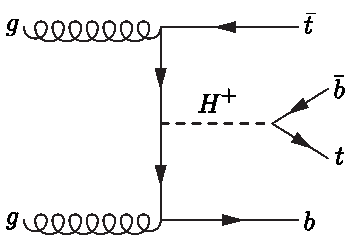
\includegraphics[width=0.5\textwidth]{HPLUSTB/feynmansmall.pdf}
    \caption{
        Leading-order Feynman diagram for the production of a heavy charged Higgs boson in association with a top antiquark and a bottom quark, as well as its decay into a top quark and a bottom antiquark.
    }
    \label{Hplustb:feynman1}
    \end{center}
\end{figure}

The signal consists in two top quarks and two bottom quarks, once of each produced in association with the $H^+$ and the other from its decay. For convenience, the typical classification for \ttbar\ events is used, based in the decay of the involved top quarks. The main decay mode for top quarks is to a $W$ and a $b$-quark, with the former decaying either leptonically (to leptons) or hadronically (to a pair of quarks). This yields to four possible diagrams depending on the decay of each top but three different types of final states with different decay rates~\cite{pdg}: the all-hadronic final state where both $W$-bosons decay hadronically (45.7\%), the dileptonic mode where both $W$-bosons decay leptonically\footnote{hadronically decaying $\tau$ leptons are included in the numbers.} (10.5\%) and the lepton+jets (semi-leptonic) final state, in which one $W$-boson decays hadronically and one leptonically (43.8\%).

In the scope of the thesis, the lepton+jets channel is studied as offers large statistics with a relatively clean topology, as the lepton in the final state allows to suppress the multijet background. Also the full event can be kinematically reconstructed, since only one neutrino is present and can be determined with the \MET. The dilepton channel was studied in the past~\acrshort{ATLASlabel} searches, with low impact in the final result. Aside, the lepton+jets channel could be further split into a resolved (low \pT) regime and a boosted regime, in order to optimise high \pT\ regimes that lead to collimated partons that cannot be resolved with the standard jet collections. The final state is depicted in Figure~\ref{Hplustb:feynman2}

\begin{figure}[htbp]
    \RawFloats
    \begin{center}
    \subfloat[]{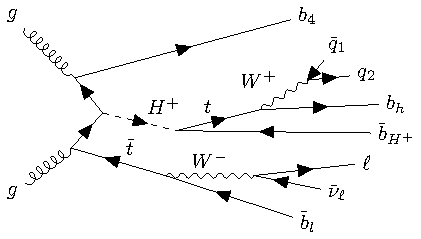
\includegraphics[width=0.47\textwidth]{HPLUSTB/feynman_had.pdf}} \quad
    \subfloat[]{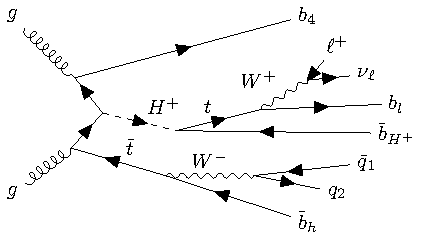
\includegraphics[width=0.47\textwidth]{HPLUSTB/feynman_lep.pdf}}
    \caption{
        Leading-order Feynman diagram for the production and decay of a heavy charged Higgs boson into a top and a bottom quark, with the former decaying hadronically (a) or leptonically (b), in the signal-lepton final state.
    }
    \label{Hplustb:feynman2}
    \end{center}
\end{figure}

The detector signature is chosen to include exactly one isolated lepton $\ell$, considering only electrons and muons. Nonetheless, the $\tau$ leptons decaying into electrons or muons are included. As six quarks are present in the final state, six jets are expected to be present in the final state with at least four of them originating from a $b$-quark. Although the recommendations available at the time were based on EMTopo jets, the performance improvements with PFlow jets would have benefited the analysis, as the $b$-tagging is one important part of the selection.

The targetted final state complexity originates from the dominant \ttbar\ production with additional jets (\ttbar+jets). In particular, \ttb\ is The main irreducible background for which an example diagram is shown in Figure~\ref{Hplustb:feynman3}. Hence, the correct modelling of this process is key for the analysis and unfortunately, it is poorly constrained by data measurements and has large theory uncertainties. 


\begin{figure}[htbp]
    \RawFloats
    \begin{center}
    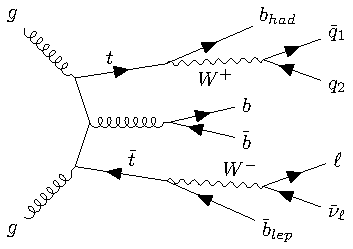
\includegraphics[width=0.5\textwidth]{HPLUSTB/feynman_ttbar.pdf}
    \caption{
        Leading-order Feynman diagram for the \ttbar\ production with a radiated $b\bar{b}$ in the single-lepton final state.
    }
    \label{Hplustb:feynman3}
    \end{center}
\end{figure}

presents the search for a charged Higgs boson produced in association with a top
quark, where the Higgs boson decays in a top-bottom pair with a single-lepton final state.
The analysis strategy is described in the first part, starting with  the event selection and
categorisation. Events are classified into different regions in order to enhance the sensitivity
to the signal and to improve the control over the SM backgrounds. The regions are designed
to be enriched in different \ttbar+jets categories: a low number of $b$-jets provides control on
the \ttbar+light category, while a request of three or more $b$-jets isolates the \ttc\ and
\ttb\ backgrounds. Regions with at least three $b$-jets are also heavily enriched in signal
and are therefore named signal regions. A boosted decision tree is used to improve the
separation between signal and background processes in the signal regions. The signal strength
is extracted with a binned profile likelihood fit, performed on the distribution of the BDT
output. The fit runs simultaneously on all regions and separately for each of the H+ mass
hypotheses. A large set of nuisance parameters is used to cover all systematic uncertainties.
They are described in the second part of the chapter, together with the results. A 95\% CL
limit is provided for the cross-section of the signal production (times the BR of the decay)
and for the $\tan\beta$ parameter of the MSSM, as a function of the signal mass. 






